\chapter{Teoremas generales}\label{chap:teoremas}

\section{Formas de onda}
	
En los circuitos eléctricos, las funciones de excitación y respuesta
son tensiones e intensidades que varían con el tiempo:
\begin{equation*}
  u=u(t)
\end{equation*}
\begin{equation*}
  i=i(t)
\end{equation*}
Estas funciones pueden representarse de forma gráfica o analítica. En
ambos casos, esa relación funcional se conoce mediante el nombre de
\textbf{forma de onda}. Las formas de onda pueden clasificarse según
(de manera análoga a lo indicado en la Sección~\ref{sec:cc-ca}):
\begin{itemize}
\item \textbf{Signo de la magnitud}:
  \begin{itemize}
  \item \textbf{Unidireccionales}: la magnitud que la representa
    siempre tiene una única polaridad (signo constante, aunque el
    valor puede ser constante o variable)
  \item \textbf{Bidireccionales}: la magnitud toma valores positivos y
    negativos (signo variable con el tiempo)
  \end{itemize}
\item \textbf{Repetición del valor de la magnitud}:
  \begin{itemize}
  \item \textbf{Periódicas}: el valor de la magnitud se repite de
    forma regular
  \item \textbf{No periódicas}: el valor de la magnitud varía de forma
    arbitraria con el tiempo
  \end{itemize}
\end{itemize}

\subsection{Formas de onda básicas}
En el estudio de la teoría de circuitos, son de especial interés las
formas de onda en escalón, rampa, pulsos y triangular.
	
\subsection{Función escalón}
Esta función vale 0 para tiempos negativos ($t<0$) y un valor
constante $K$ para tiempos positivos ($t>0$), como se muestra en la
Figura~\ref{fig:escalon}. Por tanto, su expresión matemática es:
\begin{equation}
  \boxed{f(t) = %
    \begin{cases}
      0 & t < 0\\
      K & t \geq 0
    \end{cases}}
\end{equation}
	
\begin{figure}[H]
  \centering 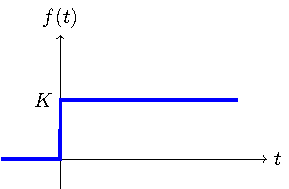
\includegraphics[height=3cm]{../figs/escalon.pdf}
  \caption{Función escalón en el origen de tiempos}
  \label{fig:escalon}
\end{figure}
	
Cuando $K = 1$, la función recibe el nombre de \textbf{escalón
  unitario}. En general, se puede considerar cualquier función escalón
como el producto de una constante (denominada \textit{amplitud}) por
la función escalón unitario.  En general, multiplicar una función por
la función escalón unitario se asocia a asignar el valor 0 para $t<0$
y no modifica la función para $t>0$.
	
\subsection{Función pulso rectangular}
	
Esta forma de onda es muy habitual en electrónica, y se representa en
la Figura~\ref{fig:pulso}. Su expresión matemática viene dada por:
\begin{equation}
  \boxed{f(t) = %
    \begin{cases}
      0 & t < 0\\
      K & 0 \leq t \leq W\\
      0 & t>W
    \end{cases}}
\end{equation}
\begin{figure}[H]
  \centering 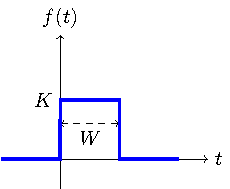
\includegraphics[height=3cm]{../figs/pulso.pdf}
  \caption{Función pulso rectangular}
  \label{fig:pulso}
\end{figure}
	
El valor $W$ se conoce como \textbf{anchura/duración del pulso}.
	
\subsection{Función rampa}
La forma de esta función es la indicada en la Figura~\ref{fig:rampa},
expresada de manera matemática de la siguiente forma:
\begin{equation}
  \boxed{f(t) = %
    \begin{cases}
      0 & t < 0\\
      m \cdot t  & t \geq 0
    \end{cases}}
\end{equation}
\begin{figure}[H]
  \centering 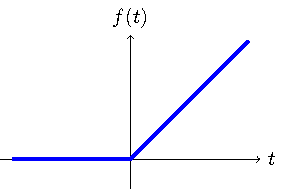
\includegraphics[height=3cm]{../figs/rampa.pdf}
  \caption{Función rampa}
  \label{fig:rampa}
\end{figure}
El valor de $m$ es la pendiente de la rampa.
	
\subsection{Función triangular}
La forma de esta función es la indicada en la
Figura~\ref{fig:triangular}, expresada de manera matemática de la
siguiente forma:
\begin{equation}
  \boxed{
    f(t) = %
    \begin{cases}
      0 & t < -W/2\\
      m \cdot (t + W/2)  & -W/2 \leq t \leq 0\\
      -m \cdot (t - W/2)  & 0 \leq t \leq W/2\\
      0  & t > W/2
    \end{cases}}
\end{equation}
\begin{figure}[H]
  \centering 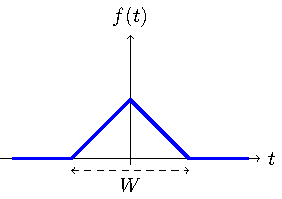
\includegraphics[height=3cm]{../figs/triangular.pdf}
  \caption{Función triangular}
  \label{fig:triangular}
\end{figure}
	
\subsection{Retraso del origen de tiempos}
Una forma de onda puede retrasarse en el tiempo si se desplaza el eje
de ordenadas en una cantidad $-t_0$. La Figura~\ref{fig:retraso}
muestra diversos ejemplos de las formas de onda básicas.
\begin{figure}[H]
  \centering \subfloat[Escalón
  retrasado]{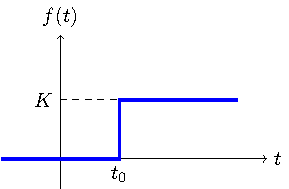
\includegraphics[height=3cm]{../figs/escalon_t0.pdf}}\hfil
  \subfloat[Pulso retrasado]{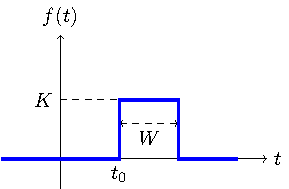
\includegraphics[height=3cm]{../figs/pulso_t0.pdf}}\\
  \subfloat[Rampa
  retrasada]{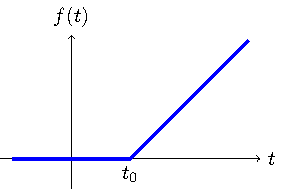
\includegraphics[height=3cm]{../figs/rampa_t0.pdf}}\hfil
  \subfloat[Triangular
  retrasada]{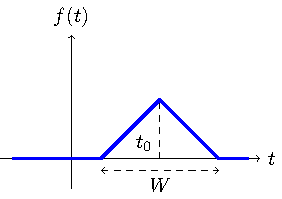
\includegraphics[height=3cm]{../figs/triangular_t0.pdf}}
  \caption{Formas de onda básicas retrasadas}
  \label{fig:retraso}
\end{figure}
	
	
\section{Teoremas de linealidad}
	
Un circuito eléctrico es lineal si los elementos pasivos y activos que
incluye son lineales:
\begin{itemize}
\item Un elemento pasivo es lineal si la relación entre la tensión
  entre sus terminales y la corriente que lo recorre es lineal:
  resistencias, condensadores y bobinas.
\item Una fuente dependiente es lineal si su salida (tensión o
  corriente) tiene una relación lineal con la magnitud del circuito de
  la que depende.
\end{itemize}
Un circuito lineal tiene dos propiedades:
\begin{itemize}
\item Homogeneidad o \textbf{proporcionalidad}: Sea $y(t)$ la
  respuesta de un circuito lineal a una excitación $x(t)$. Si la
  excitación es multiplicada por una constante, $K\cdot x(t)$, la
  respuesta del circuito será modificada por la misma constante,
  $K \cdot y(t)$.
\item Aditividad o \textbf{superposición}: La respuesta de un circuito
  lineal a varias fuentes de excitación actuando simultáneamente es
  igual a la suma de las respuestas que se tendrían cuando actuase
  cada una de ellas por separado:
  \begin{equation*}
    y(t)=\sum_i y_i(t)
  \end{equation*}
\end{itemize}

\subsection{Teorema de proporcionalidad}
\label{sec:proporcionalidad}

Este teorema es consecuencia de la propiedad de homogeneidad. Sea $y(t)$ la respuesta de un circuito lineal a una excitación $x(t)$.  Si la excitación es multiplicada por una constante, $K \cdot x(t)$, la respuesta del circuito será modificada por la misma constante, $K \cdot y(t)$.

\begin{figure}[H]
  \centering
  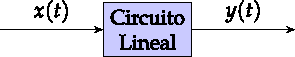
\includegraphics{../figs/proporcionalidad.pdf}
  \caption{Teorema de Proporcionalidad}
  \label{fig:superposicion_cc}
\end{figure}

\subsection{Teorema de superposición}
\label{sec:superposicion}

Es consecuencia de la propiedad de superposición de los circuitos
lineales: la respuesta total debida a varias fuentes de
excitación actuando simultáneamente es igual a la suma de las
respuestas que se tendrían cuando actuase cada una de ellas por
separado:
\begin{equation*}
  y(t) = \sum_i y_i(t)
\end{equation*}
    
El teorema dice así: \textit{En una red formada por generadores
  (dependientes e independientes) y resistencias, la corriente en una
  rama o la tensión en un nudo, cuando todos los generadores actúan
  simultáneamente, es la suma de las corrientes o las tensiones que
  crearía cada generador \textbf{independiente} si actuase solo
  (individualmente) sobre el circuito}

\begin{figure}[H]
  \centering
  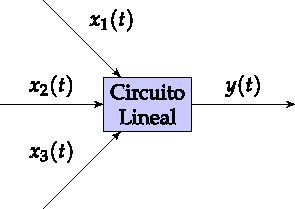
\includegraphics{../figs/superposicion.pdf}
  \caption{Teorema de Superposicion}
  \label{fig:superposicion}
\end{figure}

El procedimiento para analizar un circuito eléctrico mediante
superposición es el siguiente:
\begin{enumerate}
\item Se ``apagan'' todas las fuentes \textbf{independientes} del
  circuito menos una:
  \begin{itemize}
  \item Las fuentes de tensión se sustituyen por un cortocircuito
    ($U = 0$)
  \item Las fuentes de corriente se sustituyen por un circuito abierto
    ($I = 0$)
  \item Las fuentes \textbf{dependientes} \textbf{no} se modifican
  \end{itemize}
\item Se analiza el circuito, obteniendo la respuesta individual a la
  fuente que permanece activa.
\item Se repite este procedimiento para cada una de las fuentes
  \textbf{independientes} del circuito.
\item La respuesta total del circuito es la suma de las respuestas
  individuales.
\end{enumerate}

Para seguir este procedimiento, hay que tener en cuenta una serie de
observaciones:
\begin{itemize}
\item \textbf{Siempre} hay que aplicar este método cuando en un
  circuito conviven fuentes de \textbf{diferente frecuencia} (ya sea
  diferente pulsación, o porque existan fuentes de corriente continua
  y corriente alterna).
\item En el caso de fuentes de corriente alterna \textbf{sinusoidal},
  la respuesta debe expresarse en el \textbf{dominio del
    tiempo}. \textbf{No} se pueden \textbf{sumar} los \textbf{fasores}
  que corresponden a \textbf{frecuencias diferentes}.
\item En el primer paso del procedimiento, se pueden agrupar las
  fuentes que funcionan a la misma frecuencia y calcular la respuesta
  del circuito en esa frecuencia.
\end{itemize}

Hay que resaltar que el principio de superposición se aplica a \textbf{tensiones} y
\textbf{corrientes}, pero \textbf{no} a potencias, como se comprobará en los siguientes apartados.

\begin{example}\label{ex:superposicion_ca}
  \textbf{El circuito de la Figura~\ref{fig:superposicion1} se
    encuentra en régimen permanente. Determinar analíticamente la
    expresión de $i(t)$}

  Datos:
  $e_1(t) = {50 \sin(1000 t)}\,V;\; e_2(t) = {30}\,V;\; R_1 =
  6\,\Omega;\; R_2 = {6}{\Omega};\; L = {8}{mH};\; C = {10}{\mu F}$

\begin{figure}[H]
  \centering
  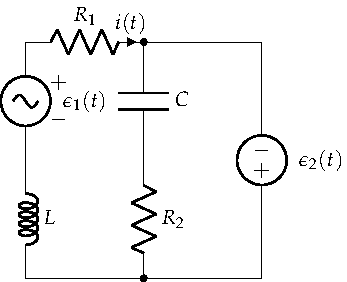
\includegraphics[width=0.25\linewidth]{../figs/superposicion1.pdf}
  \caption{Ejemplo~\ref{ex:superposicion_ca}}
  \label{fig:superposicion1}
\end{figure}

Se aplica el teorema de superposición.

\underline{Actúa la fuente de corriente alterna}

\begin{figure}[H]
  \centering
  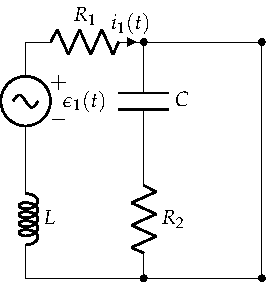
\includegraphics[width=0.25\linewidth]{../figs/superposicion1_AC.pdf}
  \caption{Circuito cuando actúa la fuente de alterna}
  \label{fig:superposicion1_AC}
\end{figure}

La rama $R_2 - C$ está cortocircuitada y, por tanto, se puede
prescindir de ella:

\begin{align*}
  \overline{Z_1} &= R_1 + \mathrm{j}\,X_L = 6 + \mathrm{j}8\Omega\\
  \overline{I'} &= \dfrac{\overline{\epsilon_1}}{\overline{Z_1}} = \dfrac{\frac{50}{\sqrt{2}}\phase{0^\circ}}{6+\mathrm{j}8}=3.54\phase{-53.1301^\circ} A
\end{align*}

En el dominio del tiempo es:

\begin{equation*}
  i(t)' = 5\sin(1000t - 0.9273) A
\end{equation*}

\underline{Actúa la fuente de corriente continua}

\begin{figure}[H]
  \centering
  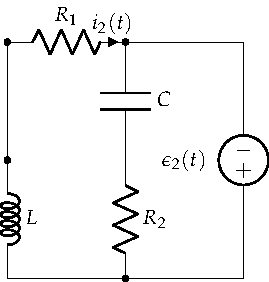
\includegraphics[width=0.25\linewidth]{../figs/superposicion1_DC.pdf}
  \caption{Circuito cuando actúa la fuente de continua}
  \label{fig:superposicion1_DC}
\end{figure}

En este circuito se sustituye la bobina por un cortocircuito y el
condensador por un circuito abierto. En consecuencia:

\begin{equation*}
  i''(t) = \dfrac{\epsilon_2(t)}{R_1}=\dfrac{30}{6} = {5}A
\end{equation*}

Por tanto:

\begin{equation*}
  i(t) = i'(t) + i''(t) = 5 + 5\sin(1000t - 0.9273) A
\end{equation*}

\end{example}

\subsubsection{Potencia disipada en una resistencia}
Supóngase que $i(t) = i_1(t) + i_2(t)$, donde
$i_1(t)=\sqrt{2}I_{1}\,\sin(\omega_1\,t)$ e
$i_2(t)=\sqrt{2}I_{1}\,\sin(\omega_2\,t)$. La potencia instantánea
disipada en una resistencia $R$ es:
\begin{align*}
  p(t) &= R \cdot i^2(t) = R \cdot (i_1(t) + i_2(t))^2\\xs
  &=R \cdot (i_1^2(t) + i_2^2(t) + 2\cdot i_1(t) \cdot i_2(t))
\end{align*}
es decir, la potencia instantánea disipada en la resistencia no es la
suma de las potencias individuales, $p(t) \neq p_1(t) + p_2(t)$.

No obstante, si calculamos la potencia activa (que, como vimos, es el valor medio de la potencia instantánea), podemos obtener un resultado útil:
\begin{align*}
  P_R &=\dfrac{1}{T}\int_0^{T}R\cdot i^2(t)\,dt=\dfrac{R}{T}\int_0^T\left[ \sqrt{2}\,I_{1}\,\sin(\omega_1\,t)+\sqrt{2}\,I_{2}\,\sin(\omega_2\,t)\right]^2\,dt=\\
  & = \dfrac{R}{T}\left[ \int_0^T (\sqrt{2}\,I_{1})^2\,\sin^2(\omega_1\,t)\,dt + \int_0^T (\sqrt{2}\,I_{1})^2\,\sin^2(\omega_2\,t)\,dt + 
    \int_0^T 2\,\sqrt{2}\,I_{1}\,\sqrt{2}\,I_{2}\,\underbrace{\sin(\omega_1\,t)\,\sin(\omega_2\,t)}_{\frac{1}{2}\,\left[\cos(A-B)-\cos(A+B)\right]}\,dt \right]
\end{align*}
donde $T$ es el periodo de la función $i(t)$\footnote{$i(t)$ es una
  función periódica no senoidal, y su periodo se corresponde con el
  mínimo común múltiplo de los periodos de las funciones que la
  forman, es decir: $T=k_1\cdot T_1=k_2\cdot T_2$, siendo $k_1$ y
  $k_2$ números enteros.}.

Evaluando cada integral de manera independiente, se obtiene que la
potencia disipada en la resistencia es:
\begin{equation*}
  P_R=R\cdot I_1^2+R\cdot I_2^2 = P_{R1} + R_{R2}
\end{equation*}
En general, si la corriente tuviese más componentes, o alguna de ellas
fuera continua, la potencia disipada por una resistencia es:
\begin{equation}\label{eq:P_R_superposicion}
  \boxed{P_R=R\cdot\left(I_{cc}^2+I_1^2+I_2^2+...+I_n^2 \right)}
\end{equation}
\begin{remark}
  Se presenta aquí el desarrollo de las integrales
  anteriores. Evaluando cada integral de manera independiente:
  \begin{align*}
    &\dfrac{R}{T} \int_0^T (\sqrt{2}\,I_{1})^2\,\sin^2(\omega_1\,t)dt=\dfrac{2\,R\,I_{1})^2}{T}\int_0^T\dfrac{1-\cos(2\,\omega_1\,t)}{2}dt=\\
    &=\dfrac{2\,R\,I_{1}^2}{T}\left[\int_0^T\dfrac{1}{2}dt-\cancelto{0}{\int_0^T \dfrac{\cos(2\,\omega_1\,t)}{2}dt}\right]=R\cdot I_1^2
  \end{align*}
  De forma análoga, la segunda integral da por resultado
  $R\cdot I_2^2$. Y la tercera integral:
  \begin{equation*}
    \int_0^T 2\,\sqrt{2}\,I_{1}\, \sqrt{2}\,I_{2}\,\underbrace{\sin(\omega_1\,t)\,\sin(\omega_2\,t)}_{\frac{1}{2}\,\left[\cos(A-B)-\cos(A+B)\right]}\,dt=\dfrac{1}{2}\,4\,I_1\,I_2\,\left[\int_0^T\cos(\omega_1-\omega_2)\,t\,dt-\int_0^T\cos(\omega_1+\omega_2)\,t\,dt\right]
  \end{equation*}
  haciendo
  $\omega_1-\omega_2=\omega'=2\,\pi\left(\frac{1}{T_1}-\frac{1}{T_2}
  \right)=2\,\pi\left(\frac{k_1}{T}-\frac{k_2}{T}\right)=2\,\pi\,k'\,\frac{1}{T}$,
  donde $k'=k_1-k_2$. Del mismo modo,
  $\omega_1+\omega_2=\omega''=2\,\pi\,k''\,\frac{1}{T}$, donde
  $k''=k_1+k_2$. Con estos cambios, la integral anterior queda:
  \begin{align*}
    &2\,I_1\,I_2\,\left[\int_0^T\cos(\omega'\,t)\,dt-\int_0^T\cos(\omega''\,t)\,dt\right]=\\
    =2\,I_1\,I_2\,&\left[\cancelto{0}{\int_0^T \cos\left(2\pi k'\dfrac{t}{T}\right)\,dt}-\cancelto{0}{\int_0^T\cos\left(2\pi k''\dfrac{t}{T}\right)\,dt}\right]=0
  \end{align*}
\end{remark}


\subsubsection{Potencia entregada por una fuente de tensión}
    
Supóngase que $i(t) = i_1(t) + i_2(t)$, donde
$i_1(t)=\sqrt{2}I_{1}\,\sin(\omega_1\,t+\theta_{i1})$ e
$i_2(t)=\sqrt{2}I_{1}\,\sin(\omega_2\,t+\theta_{i2})$. La potencia
instantánea entregada por una fuente de tensión de fem
$\epsilon(t)=\sqrt{2}\,E\,\sin(\omega_1\,t)$ es:
\begin{equation*}
  p(t) = e(t)\cdot i(t) = \sqrt{2}\,E\, \sqrt{2}\,I_{1}\,\sin(\omega_1\,t)\,\sin(\omega_1\,t+\theta_{i1}) +\sqrt{2}\,E\, \sqrt{2}\,I_{2}\,\sin(\omega_1\,t)\,\sin(\omega_2\,t+\theta_{i2})
\end{equation*} 
En este caso, se tiene que $e(t)$ es una función senoidal de periodo
$T_1$, mientras que $i(t)$ es una función periódica no senoidal de
periodo $T=m.c.m.(T_1,T_2)$.

El valor medio de la potencia instantánea se corresponde con la
potencia real (activa) entregada:
\begin{align*}
  P&=\dfrac{1}{T}\int_0^{T}\left( \sqrt{2}\,E\,\sqrt{2}\, I_{1}\,\underbrace{\sin(\omega_1\,t)\,\sin(\omega_1\,t+\theta_{i1}}_{\frac{1}{2}\left[\cos(A-B)-\cos(A+B)\right]}) + \sqrt{2}\,E\,\sqrt{2}\, I_{2}\,\cancelto{\text{0, si $\theta_{i2}=0$}}{\sin(\omega_1\,t)\,\sin(\omega_2\,t+\theta_{i2})}\right)dt=\\
  =&\dfrac{1}{T}\int_0^T \cancel{2}\,E\,I_{1}\dfrac{\cos(-\theta_{i1})-\cos(2\,\omega_1\,t+\theta_{i1})}{\cancel{2}}dt =\dfrac{1}{T}\int_0^T E\,I_{1}\,{\cos(\theta_{i1})}\,dt-\dfrac{1}{T}\int_0^T E\,I_{1}\,\cancelto{0}{{\cos(2\,\omega_1+\theta_{i1})}}\,dt
\end{align*}
por lo que la potencia entregada por la fuente de tensión es:
\begin{equation}\label{eq:P_E_superposicion}
  \boxed{P=E\,I_1\,\cos(\theta_{i1})}
\end{equation}
es decir, que a efectos de potencia, solo actúa la componente de la
intensidad que tiene \textbf{la misma frecuencia} que el generador de
tensión.

\subsubsection{Potencia entregada por un generador de intensidad}

Sea la corriente entregada por la fuente
$i(t)=\sqrt{2}\,I_g\,\sin(\omega_1\,t)$, y la tensión
$u(t)=\sqrt{2}\,U_{1}\,\sin(\omega_1\,t+\theta_{u1})+\sqrt{2}\,U_{2}\,\sin(\omega_2\,t+\theta_{u2})$. La
potencia instantánea es:
\begin{align*}
  p(t) = u(t)\cdot i(t) = \sqrt{2}\,U_{1}\, \sqrt{2}\,I_g\,\sin(\omega_1\,t)\,\sin(\omega_1\,t+\theta_{u1}) + \sqrt{2}\,U_{2}\, \sqrt{2}\,I_g\,\sin(\omega_1\,t)\,\sin(\omega_2\,t+\theta_{u2})
\end{align*} 
Como en los casos anteriores, $T=m.c.m.(T_1,T_2)$, y la potencia
entregada por el generador es:
\begin{equation*}
  P=\dfrac{1}{T}\int_0^T \left[\sqrt{2}\,U_{1}\, \sqrt{2}\,I_g\,\sin(\omega_1\,t)\,\sin(\omega_1\,t+\theta_{u1})+\sqrt{2}\,U_{2}\, \sqrt{2}\,I_g\,\sin(\omega_1\,t)\,\sin(\omega_2\,t+\theta_{u2}) \right] dt
\end{equation*}
integral que, al desarrollarla, incluye los mismos términos nulos que
en los casos anteriores, por lo que el resultado es:
\begin{equation}\label{eq:P_I_superposicion}
  \boxed{P=U_1\,I_g\,\cos(\theta_{u1})}
\end{equation}
    
\begin{remark}
  Las integrales que se han ido anulando son \textbf{señales
    ortogonales en un periodo}. Dos señales son ortogonales si cumplen
  la siguiente ecuación:
  \begin{equation*}
    <f_1, f_2>_T = \int_T f_1(t) \cdot f_2(t) dt = 0
  \end{equation*}
  Son señales ortogonales todas las funciones sinusoidales de
  diferente frecuencia, así como las funciones sinusoidales con
  funciones continuas. Por tanto, en los casos que aparecen en teoría
  de circuitos, las
  expresiones~\eqref{eq:P_R_superposicion}--\eqref{eq:P_I_superposicion}
  serán siempre válidas.
\end{remark}

	
\begin{example}\label{ex:superposicion_ca_potencia}
  \textbf{Determina el balance de potencias del circuito de la Figura~\ref{fig:superposicion1} del ejemplo \ref{ex:superposicion_ca_potencia}.}

\underline{Actúa la fuente de corriente alterna}

El balance de potencias es:

\begin{align*}
  P_{R1}' &= I_1^2\cdot R_1= 3.54^2\cdot 6= {75.19}{W}\\
  P_{R2}' &= {0} W\\
  P_{\epsilon1} &= \epsilon_1 \cdot {I'}\cdot\cos(\theta_{i'}) = \dfrac{50}{\sqrt{2}}\cdot 3.54\cdot\cos(-53.1301) = 75.19 W
\end{align*}

\underline{Actúa la fuente de corriente continua}

El balance de potencias es:

\begin{align*}
  P_{R1}'' &= I_2^2 \cdot R_1=5^2\cdot 6 = {150} W\\
  P_{R2}'' &= {0} W\\
  P_{\epsilon2} &= \epsilon_2 \cdot I''\cdot\cos(\theta_{i''}) = 30\cdot 5\cdot\cos(0)  = {150} W
\end{align*}

Como las señales son ortogonales, se puede hacer el balance de
potencias conjunto con los dos circuitos:

\begin{align*}
  P_{R1} &= P_{R1}' + P_{R1}'' = 75.19+150={225.19} W\\
  P_{R2} &= P_{R2}' + P_{R2}'' = 0+0 = {0} W\\
  P_{\epsilon} &= P_{\epsilon1} + P_{\epsilon2} = 75.19 + 150={225.19} W\\
\end{align*}
\end{example}
	
\section{Teoremas de Thévenin y Norton}
Cuando el interés en el estudio de un circuito se fija en una parte
del mismo (por ejemplo, en una rama), es interesante poder separar
esta rama del resto de la red para no tener que resolver el circuito
completo cada vez que se modifican los parámetros de dicha rama.  Los
teoremas de Thévenin y Norton constituyen dos procedimientos para
sustituir el resto de la red, y hacer más simple el cálculo de
tensiones, corrientes, etc. en la rama que se desea estudiar de un
modo específico. Por tanto, resuelve el problema de sustituir una red
compleja por un circuito equivalente más simple, evitando así cálculos
repetitivos innecesarios.

\subsection{Teorema de Thévenin}
Enunciado por León Charles Thévenin en 1883, un ingeniero de
telégrafos francés, este teorema dice lo siguiente: \textit{cualquier
  \textbf{red lineal} compuesta por elementos pasivos y activos
  (dependientes o independientes) se puede sustituir, desde el punto
  de vista de unos terminales externos $A-B$, por una fuente de
  tensión $\overline{\epsilon}_{th}$ (generador de Thévenin) y una
  impedancia en \textbf{serie} $\overline{Z}_{th}$ (impedancia de
  Thévenin)}. La Figura~\ref{fig:thevenin_ca} muestra el circuito
equivalente Thévenin de una red lineal.
\begin{figure}[H]
  \centering \subfloat[Red
  lineal]{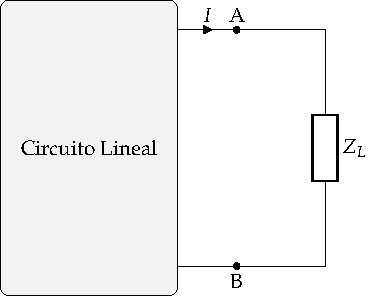
\includegraphics[width=0.32\linewidth]{../figs/CircuitoLineal_ZL.pdf}}\hfil
  \subfloat[Equivalente
  Thévenin]{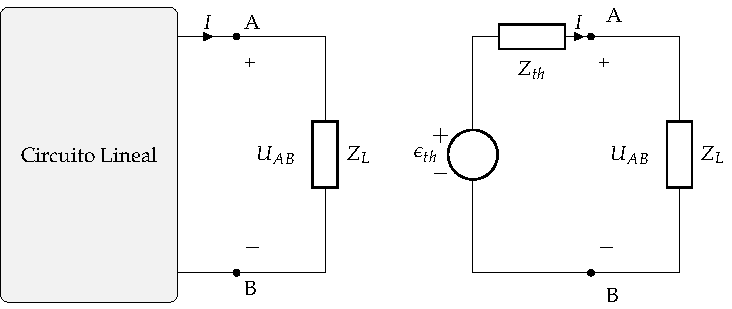
\includegraphics[width=0.29\linewidth]{../figs/EquivalenteThevenin.pdf}}
  \caption{Equivalente de Thévenin}
  \label{fig:thevenin_ca}
\end{figure}
     
    
Si ambos circuitos han de ser equivalentes, deberán dar los mismos
valores de tensión y corriente a la impedancia de carga $Z_L$. Entre
todos los valores posibles de $Z_L$, se analizan los dos casos
extremos ($Z_L \to \infty$ y $Z_L=0$):
\begin{itemize}
\item $Z_L \to \infty$: este caso significa físicamente
  \textbf{desconectar} la impedancia de carga del circuito. En esta
  situación, el dipolo de la red lineal dará una tensión en vacío o en
  circuito abierto ($U_0$) siendo $I=0$, que deberá ser idéntica a la
  que debe dar el circuito del equivalente Thévenin, donde la tensión
  entre los terminales $A-B$ es igual a $\epsilon_{th}$, ya que la
  caída de tensión en $\overline{Z}_{th}$ será nula. Por consiguiente, \textbf{el
    valor de $\epsilon_{th}$ de la red equivalente es igual a la
    magnitud $U_0$ de la red lineal que se obtiene entre los
    terminales de salida $A-B$ al desconectar la carga y dejar el
    circuito abierto}.
\item $Z_L=0$: Este caso representa un cortocircuito entre los
  terminales externos $A-B$. Denominando $I_{sc}$ a la corriente que
  circula por este cortocircuito, debe obtenerse la misma $I_{sc}$ en
  el equivalente de Thévenin, resultando, por tanto:
  \begin{equation}\label{eq:Zth}
    \overline{I}_{sc}=\dfrac{\overline{\epsilon}_{th}}{\overline{Z}_{th}}\Rightarrow
    \boxed{\overline{Z}_{th}=\dfrac{\overline{\epsilon}_{th}}{\overline{I}_{sc}}}
  \end{equation}
  es decir, \textbf{el valor de $\overline{Z}_{th}$ se obtiene como el cociente
    entre la tensión que da la red en vacío y la corriente de
    cortocircuito}. Si los generadores del circuito son todos
  independientes, el cálculo de la impedancia de Thévenin es más simple
  que lo expresado en la fórmula~\eqref{eq:Zth}, y representa el
  \textbf{valor de la impedancia que se observa entre los terminales
    $A-B$} de salida cuando se anulan los generadores internos del
  circuito (es decir, se cortocircuitan las fuentes de tensión y se
  abren las de corriente). Téngase en cuenta que, si se anulan los
  generadores, al no existir fuentes de excitación, darán lugar a una
  tensión de Thévenin $\epsilon_{th}=0$ y, si se anula
  $\epsilon_{th}$, la impedancia que se observa entre los terminales
  $A-B$, quitando la carga, coincide con $\overline{Z}_{th}$.
  \begin{remark}
    En ocasiones, calcular $I_{sc}$ puede ser complicado. Otra manera
    de determinar el valor de $\overline{Z}_{th}$ es incluyendo entre $A-B$ una
    fuente de prueba, de fem $\epsilon_0$, y haciendo el cociente
    entre:
    \begin{equation*}
      \overline{Z}_{th}=\dfrac{\overline{\epsilon}_0}{\overline{I}_{0}}
    \end{equation*}
    donde $I_{0}$ es la corriente suministrada por la fuente de
    prueba, que será función de $\epsilon_0$.
  \end{remark}
\end{itemize}
     
     
\subsection{Teorema de Norton}
Enunciado por el ingeniero estadounidense Edward Lawry Norton, de los
Laboratorios Bell, que lo publicó en un informe interno en el año
1926, se trata de la versión dual del teorema de Thévenin, diciendo lo
siguiente: En este caso, el teorema se generaliza, de manera que
\textit{cualquier \textbf{red lineal} compuesta por elementos pasivos
  y activos (dependientes o independientes) se puede sustituir, desde
  el punto de vista de unos terminales externos $A-B$, por una fuente
  de corriente $\overline{I_{N}}$ (generador de Norton) y una
  impedancia en \textbf{paralelo} $\overline{Z_{N}}$ (impedancia de
  Norton)}. Al circuito de la Figura~\ref{fig:norton1} se le denomina
equivalente Norton, y si se compara con el equivalente Thévenin, se
observa que no es más que el que resulta de sustituir una fuente de
tensión por una de corriente.
\begin{figure}[H]
  \centering \subfloat[Red
  lineal]{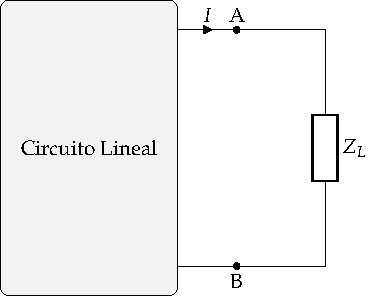
\includegraphics[width=0.35\linewidth]{../figs/CircuitoLineal_ZL.pdf}}\hfil
  \subfloat[Equivalente
  Norton]{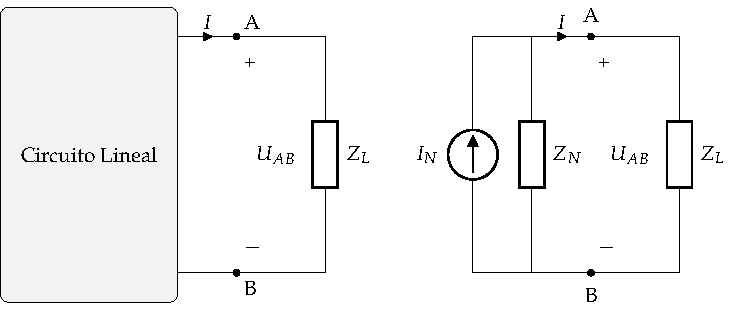
\includegraphics[width=0.3\linewidth]{../figs/EquivalenteNorton.pdf}\label{fig:norton1}}
  \caption{Equivalente de Norton}
\end{figure}

Al circuito de la Figura~\ref{fig:norton1} se le denomina
equivalente Norton, y si se compara con el equivalente Thévenin, se
observa que no es más que el que resulta de sustituir una fuente de
tensión por una de corriente donde se cumple que:
\begin{equation}
  \boxed{\overline{I}_N=\dfrac{\overline{\epsilon}_{th}}{\overline{Z}_{th}}= I_{sc}} \qquad\qquad \boxed{\overline{Z}_N=\overline{Z}_{th}}
\end{equation}
de donde se deduce que el generador de corriente de Norton es igual a
la corriente que se obtiene en la red lineal al juntar sus terminales
($Z_L=0$) y que la impedancia de Norton es el cociente entre la
tensión de vacío ($Z_L \to \infty$) y la corriente de cortocircuito de la
red (al igual que la impedancia de Thévenin).
\begin{remark}
  Gracias a la equivalencia de fuentes
  (expresión~\eqref{eq:equivalencia_fuentes}), una vez obtenido uno de
  los equivalentes se puede obtener el otro mediante una
  transformación.
\end{remark}

\begin{example}\label{ex:Th_cc}
  \textbf{Determinar el equivalente de Thévenin del circuito de la
    Figura~\ref{fig:ej_Th_cc} visto desde los terminales $A-B$, y la
    potencia que se disiparía si se conectase una resistencia de
    5$\Omega$.}
  \begin{figure}[H]
    \centering 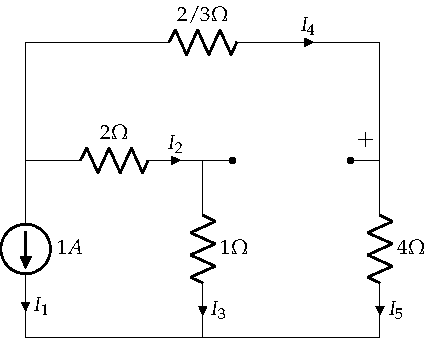
\includegraphics{../figs/ej_Th_cc1.pdf}
    \caption{Ejemplo~\ref{ex:Th_cc}}
    \label{fig:ej_Th_cc}
  \end{figure}
    
  \underline{Cálculo de $\epsilon_{th}$}
    
  Se corresponde con la caída de tensión en vacío que habría entre
  esos terminales $A-B$. Resolviendo el circuito, se obtiene que las
  corrientes son:
  \begin{align*}
    I_1&=1\,A\\
    I_2&=I_3=-14/23\,A\\
    I_4&=I_5=-9/23\,A
  \end{align*}
  y, por la 2LK:
  \begin{equation*}
    \epsilon_{th}=-I_4\,\dfrac{2}{3}+I_2\,2=\dfrac{9}{23}\cdot\dfrac{2}{3}-\dfrac{14}{23}\cdot 2=-\dfrac{22}{23}\,V
  \end{equation*}
    
  \underline{Cálculo de $R_{th}$}
    
  Al no haber fuentes dependientes, se puede obtener directamente
  calculando la resistencia equivalente vista desde los terminales
  desde los que se calcula el equivalente Thévenin cuando se
  ``anulan'' todas las fuentes. En este caso, dicha resistencia es:
  \begin{equation*}
    R_{th}=\dfrac{(\frac{2}{3}+2)\cdot(1+4)}{(\frac{2}{3}+2)+(1+4)}=\dfrac{40}{23}\Omega
  \end{equation*}
    
  \underline{Potencia de una $R=5\Omega$}
    
  Si se conecta una resistencia de 2 $\Omega$, la resistencia
  equivalente es:
  \begin{equation*}
    R_{eq}=\dfrac{40}{23}+2=\dfrac{155}{23}\Omega
  \end{equation*}
  por lo que la intensidad que circula por el circuito (alternando la
  polaridad de la fuente):
  \begin{equation*}
    I=\dfrac{\epsilon_{th}}{R_{eq}}=\dfrac{\frac{22}{23}}{\frac{155}{23}}=\dfrac{22}{155} A
  \end{equation*}
  siendo la potencia disipada por la resistencia:
  \begin{equation*}
    P=R\, I^2=5\cdot \left( \dfrac{22}{155}\right)^2=0.10\,W
  \end{equation*}
\end{example}

% \begin{example}\label{ex:th_cc_dep}
%   \textbf{Determinar el equivalente de Thévenin del circuito de la
%   Figura~\ref{fig:eq_Th_cc_dep} entre los terminales $A-B$; a partir
%   de él, hallar el valor de $U_0$.}
%   \begin{figure}[H]
%     \centering 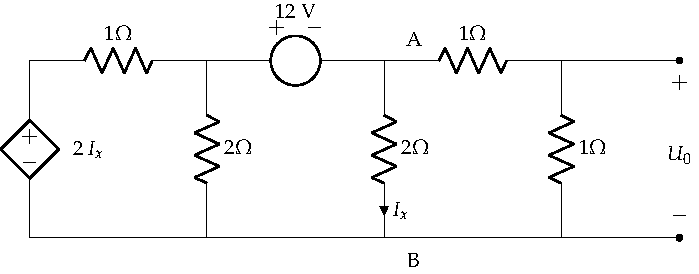
\includegraphics{../figs/eq_Th_cc_dep.pdf}
%     \caption{Ejemplo~\ref{ex:th_cc_dep}}
%     \label{fig:eq_Th_cc_dep}
%   \end{figure}
    
%   \underline{Cálculo de $\epsilon_{th}$}
    
%   Se corresponde con la caída de tensión en vacío entre los
%   terminales $A-B$, correspondiente al circuito de la
%   Figura~\ref{fig:eq_Th_cc_dep1}. Planteando el método de nudos:
%   \begin{figure}[H]
%     \centering 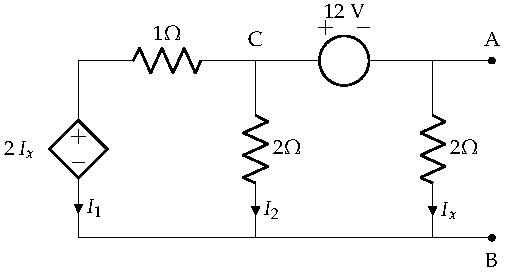
\includegraphics{../figs/eq_Th_cc_dep1.pdf}
%     \caption{Cálculo de $\epsilon_{th}$}
%     \label{fig:eq_Th_cc_dep1}
%   \end{figure}
    
%   \begin{equation*}
%     \dfrac{U_C-2\,I_x}{1}+\dfrac{U_C}{2}+\dfrac{U_C-12}{2}=0
%     \end{equation*}
%     de donde se sabe que $I_x=\frac{U_C-12}{2}$, se obtiene que:
%     \begin{equation*}
%         U_C=-6\,V
%     \end{equation*}
%     por lo que la tensión $U_{AB}=\epsilon_{th}$:
%     \begin{equation*}
%         \epsilon_{th}=U_{AB}=U_C-12=-6-12=-18\,V
%     \end{equation*}
    
%     \underline{Cálculo de $R_{th}$}
    
%     Al existir un generador dependiente, se debe determinar $R_{th}$
%     mediante un generador de prueba de valor $\epsilon_0$ situado en
%     los terminales $A-B$, y ``anulando'' la fuente dependiente, como
%     en la Figura~\ref{fig:eq_Th_cc_dep2}.
%     \begin{figure}[H]
%       \centering 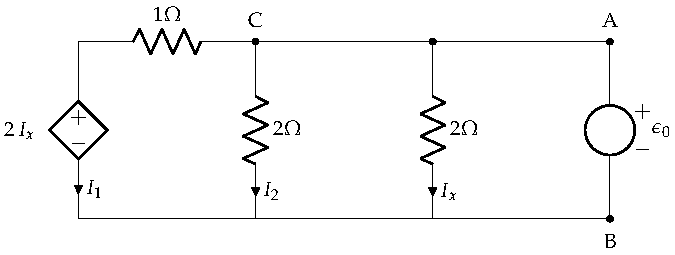
\includegraphics{../figs/eq_Th_cc_dep2.pdf}
%       \caption{Cálculo de $R_{th}$}
%       \label{fig:eq_Th_cc_dep2}
%     \end{figure}
    
%     E
    
    
%   \end{example}

\section{Teorema de la máxima transferencia de potencia}
\label{sec:teorema-max_potencia}

En equipos de transmisión--recepción, en sistemas de telecomunicación,
en amplificadores, etc., interesa que la potencia de la señal a la
salida sea máxima, es decir, que se entregue la máxima potencia a la
carga conectada en los terminales de salida.  Este teorema responde a
la siguiente pregunta: ¿\textbf{cuál es el valor de $\overline{Z}_L$ para que,
  al conectarla entre los terminales $A-B$, el circuito entregue la
  máxima potencia disponible}?

Aplicando el teorema de Thévenin (se llegaría a la misma conclusión si
se hiciera con Norton), se convierte el circuito activo en un
generador de fem $\overline{\epsilon}_{th}$ en serie con una
impedancia $\overline{Z}_{th}$ y la impedancia $\overline{Z}_L$
conectada entre $A-B$, como se muestra en la
Figura~\ref{fig:equivalenteThevenin0_ca}.
\begin{figure}[H]
  \centering 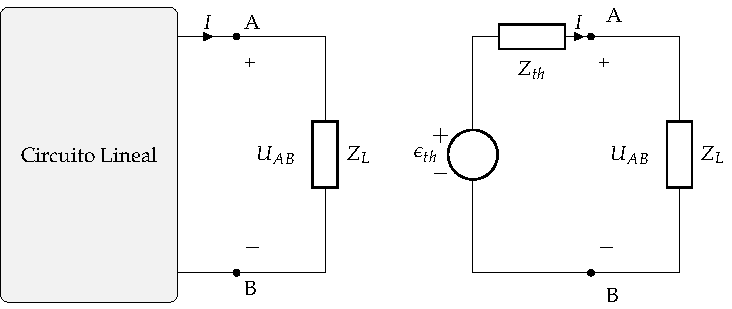
\includegraphics{../figs/EquivalenteThevenin.pdf}
  \caption{Ecuaciones del teorema de la máxima transferencia de
    potencia}
  \label{fig:equivalenteThevenin0_ca}
\end{figure}

De manera general, se tiene que:
\begin{align*}
  \overline{Z}_{th} &= R_{th} + \mathrm{j}\,X_{th}\\
  \overline{Z}_L &= R_L + \mathrm{j}\,X_L
\end{align*}
Por tanto, la corriente que circula por el circuito es:
\begin{equation*}
  \overline{I} = \frac{\overline{\epsilon}_{th}}{\overline{Z}_{th} + \overline{Z}_L}
\end{equation*}
cuyo módulo es

\begin{equation*}
  I=\frac{\epsilon_{th}}{\sqrt{(R_L+R_{th})^2+(X_L+X_{th})^2}}
\end{equation*}

Por definición, la potencia consumida por la carga $Z_L$ (la que hay que
maximizar), es:
\begin{equation*}
  P_L= I^2 \cdot R_L\Rightarrow P_L = \dfrac{\epsilon_{th}^2}{{(R_L+R_{th})^2+(X_L+X_{th})^2}} \cdot R_L
\end{equation*}
y, teniendo en cuenta las condiciones para obtener el valor máximo
$\left(\diffp{P_L}{X_L} = 0;\;\; \diffp{P_L}{R_L} = 0\right)$, se
obtiene que:
\begin{itemize}
\item \textbf{Condición de la reactancia:}
  \begin{equation}\label{eq:XL_maxpotencia}
    \diffp{P_L}{X_L} = \epsilon^2_{th} \cdot R_L \cdot \left[\frac{-1}{\left((R_L + R_{th})^2 + (X_L + X_{th})^2\right)^2} \cdot 2 \cdot (X_L + X_{th})\right]=0\Rightarrow \boxed{X_L = - X_{th}}
  \end{equation}
\item \textbf{Condición de la resistencia:} simplificando la expresión
  de la potencia al tener en cuenta la
  ecuación~\eqref{eq:XL_maxpotencia}, y calculando la derivada
  parcial:
  \begin{equation}\label{eq:R_maxpotencia}
    \diffp{P_L}{R_L} = \epsilon^2_{th} \cdot \left[\frac{1}{(R_L + R_{th})^2} - 2 \cdot \frac{R_L}{(R_L + R_{th})^3}\right]= \frac{\epsilon^2_{th} \cdot (R_{th} - R_L)}{(R_L + R_{th})^3}=0\Rightarrow \boxed{R_L = R_{th}}
  \end{equation}
\end{itemize}
Por tanto, la impedancia de carga que hay que conectar entre los
terminales $A-B$ del equivalente de Thévenin del circuito lineal para
obtener la máxima potencia disponible es:
\begin{equation}
  \boxed{\overline{Z}_L = \overline{Z}_{th}^*=R_{th}-\mathrm{j}\,X_{th}}
\end{equation}
siendo la máxima potencia disponible en la carga:
\begin{equation}
  \left.
    \begin{matrix}
      \overline{Z}_L = \overline{Z}_{th}^*\\
      P_L = \dfrac{\epsilon_{th}^2}{{(R_L+R_{th})^2+(X_L+X_{th})^2}} \cdot R_L
    \end{matrix} \right\}\rightarrow
  \boxed{P_L = \frac{\epsilon^2_{th}}{4 R_{th}}}
\end{equation}


Si la impedancia de carga es resistiva pura (figura \ref{fig:thevenin-resistencia}), la potencia en la carga es:
\begin{equation}
  P_L = \frac{\epsilon^2_{th}}{(R_{th} + R_L)^2 + X_{th}^2} \cdot R_L
\end{equation}

\begin{figure}[H]
  \centering
  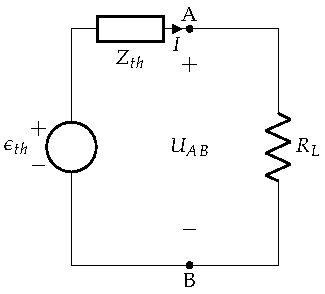
\includegraphics[height=4cm]{../figs/EquivalenteThevenin_RL.pdf}
  \caption{Circuito equivalente de Thévenin alimentando una carga resistiva.}
  \label{fig:thevenin-resistencia}
\end{figure}

En esta ecuación únicamente se puede aplicar la condición $\diff{P_L}{R_L} = 0$, de la que obtenemos:
\begin{align*}
      R_L &= |\overline{Z}_{th}| = \sqrt{R_{th}^2 + X_{th}^2}\\
      P_L &= \frac{\epsilon^2_{th}}{2(R_L + R_{th})}
\end{align*}

\begin{remark}
  Los generadores equivalentes de Thévenin, Norton y los resultados
  del teorema de la máxima transferencia de potencia solo son válidos
  para la frecuencia a la que se obtienen.
\end{remark}

\begin{example}\label{ex:th_ca}
  \textbf{En el circuito de la Figura~\ref{fig:thevenin6}, calcular:
    \begin{itemize}
    \item La fuerza electromotriz del generador equivalente de
      Thévenin respecto de A y B, $\overline{\epsilon}_{th}$
    \item La impedancia del generador equivalente de Thévenin respecto
      de A y B, $\overline{Z}_{th}$
    \item La impedancia de carga que se debe conectar entre A y B para
      conseguir la máxima potencia disponible
    \item La potencia activa entregada entre A y B cuando se conecta
      cada una de las siguientes impedancias de carga:
      \begin{itemize}
      \item $\overline{Z}_L = \overline{Z}_{th}$
      \item $\overline{Z}_L = R_{th}$ (parte resistiva de
        $\overline{Z}_{th}$)
      \item $\overline{Z}_L = \mathrm{j} X_{th}$ (parte reactiva de
        $\overline{Z}_{th}$)
      \item Impedancia calculada en el apartado anterior
      \end{itemize}
    \end{itemize}}

  Datos:
  $\; \overline{Z}_1 = 3 + \mathrm{j}4\,\Omega;\; \overline{Z}_2 = 2 +
  \mathrm{j}\,\Omega;\; \overline{\epsilon}_g =
  10\phase{30^{\circ}}\,\si{\volt}; \; \overline{I}_g =
  2\phase{15^{\circ}}\,\si{\ampere};\; \beta = 5\,\Omega$

\begin{figure}[H]
  \centering 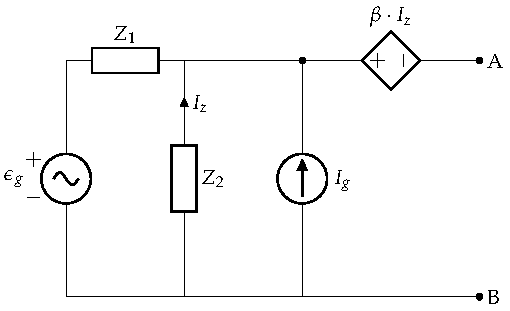
\includegraphics{../figs/thevenin6.pdf}
  \caption{Ejemplo~\ref{ex:th_ca}}
  \label{fig:thevenin6}
\end{figure}

Para calcular la \textit{fem} del generador equivalente de Thévenin,
se calcula la tensión en circuito abierto. Por 1LK, se tiene que:
\begin{equation*}
  \overline{I}_g + \overline{I}_Z + \overline{I}_{Z1} = 0 
\end{equation*}
y, aplicando 2LK:
\begin{align*}
  &- \overline{I}_Z \cdot \overline{Z}_2 = \overline{\epsilon}_g - \overline{I}_{Z1} \cdot \overline{Z}_1\\
  &\overline{U}_{AB} = - \beta \cdot \overline{I}_Z - \overline{I}_Z \cdot \overline{Z}_2
\end{align*}
Combinando estas ecuaciones, se obtiene:
\begin{equation*}
  \overline{U}_{AB}=\overline{\epsilon}_{th} = (\beta + \overline{Z}_2) \, \dfrac{\overline{\epsilon}_g + \overline{I}_g \cdot \overline{Z}_1}{\overline{Z}_1 + \overline{Z}_2} = (5+2+\mathrm{j})\cdot\dfrac{10\phase{30^\circ}+[(2\phase{15^\circ})\cdot (3+\mathrm{j}4)]}{3 + \mathrm{j}4+2 + \mathrm{j}}= \boxed{\vphantom{\frac{a}{a}} 18.90\phase{12.195^\circ}\,\si{\volt}} 
\end{equation*}

Para calcular la impedancia equivalente de Thévenin, se apagan las
fuentes independientes y se conecta un generador de prueba en A-B,
como en la Figura~\ref{fig:thevenin6_zth}:
\begin{figure}[H]
  \centering
  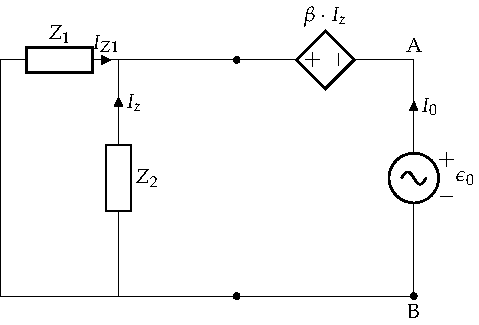
\includegraphics[width=0.5\linewidth]{../figs/thevenin6_fuenteprueba.pdf}
  \caption{Cálculo de $\overline{Z}_{th}$}
  \label{fig:thevenin6_zth}
\end{figure}

Por la 1LK:
\begin{equation*}
  \overline{I}_0 + \overline{I}_Z + \overline{I}_{Z1} = 0
\end{equation*}
y por la 2LK:
\begin{align*}
  &\overline{I}_Z \cdot \overline{Z}_2 = \overline{I}_{Z1} \cdot \overline{Z}_1\\
  &\overline{\epsilon}_0 = - \beta \cdot \overline{I}_Z - \overline{I}_Z \cdot \overline{Z}_2
\end{align*}

Combinando las ecuaciones, se llega a que:
\begin{equation*}
  \overline{Z}_{th} = \dfrac{\overline{\epsilon}_0}{\overline{I}_0} = \dfrac{\overline{Z}_1\,(\beta + \overline{Z}_2)}{\overline{Z}_1+\overline{Z}_2}=\dfrac{(3+\mathrm{j}4)\cdot (5+1+\mathrm{j})}{3+\mathrm{j}4+1+\mathrm{j}} = \boxed{\vphantom{\frac{a}{a}} 5\phase{16.2602^\circ}\,\Omega}
\end{equation*}

Finalmente, para calcular la potencia en la carga A-B, obtenemos la corriente que circula por el circuito:

  \[
    \overline{I} = \dfrac{\overline{\epsilon}_{th}}{\overline{Z}_{th} + \overline{Z}_L}
  \]

A continuación, calculamos la potencia en la impedancia $Z_L$:
  
\begin{equation*}
  P_{AB} = I^2 \cdot \Re\{\overline{Z}_L\}
\end{equation*}

Sustituyendo valores:
\begin{itemize}
\item Para $\overline{Z}_L = \overline{Z}_{th}$,
  $\;P_{AB} = \qty{17.15}{\watt}$
\item Para $\overline{Z}_L = R_{th}$, $\;P_{AB} = \qty{18.22}{\watt}$
\item Para $\overline{Z}_L = \mathrm{j}X_{th}$,
  $\;P_{AB} = \qty{0}{\watt}$
\item Para $\overline{Z}_L = \overline{Z}_{th}^*$,
  $\;P_{AB} = \qty{18.61}{\watt}$
\end{itemize}

Se comprueba que el máximo valor se obtiene cuando se conecta la
impedancia de Thévenin conjugada.

\end{example}
	
\section{\textsuperscript{TC2} Teoremas de reciprocidad y sustitución}
\label{sec:orgaf3c617}

\subsection{Teorema de reciprocidad}
\label{sec:teorema-reciprocidad}

Sea un circuito pasivo alimentado por una fuente de tensión en su entrada, y con un cortocircuito en la salida (figura \ref{fig:teorema-reciprocidad-tension1}). La corriente de cortocircuito que circula por esta rama en la salida es idéntica a la corriente que circularía si se intercambian las posiciones de la fuente y el cortocircuito (figura \ref{fig:teorema-reciprocidad-tension2}). Este resultado es consecuencia de la simetría de la matriz de impedancias de un circuito pasivo.

\begin{figure}[H]
  \centering
  \subfloat[Fuente de tensión en la entrada]{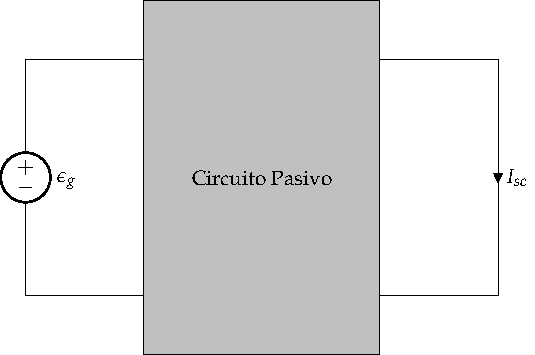
\includegraphics[height=4cm]{../figs/TeoremaReciprocidadTension1.pdf}\label{fig:teorema-reciprocidad-tension1}}\hspace{2cm}
  \subfloat[Fuente de tensión en la salida]{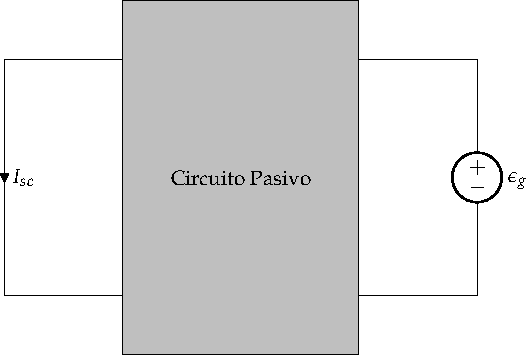
\includegraphics[height=4cm]{../figs/TeoremaReciprocidadTension2.pdf}\label{fig:teorema-reciprocidad-tension2}}
  \caption{Teorema de reciprocidad aplicado a un circuito alimentado por una fuente de tensión.}
  \label{fig:teorema-reciprocidad-tension}
\end{figure}

Este teorema se puede aplicar también a un circuito pasivo alimentado por una fuente de corriente en la entrada con un circuito abierto en la salida (figura \ref{fig:teorema-reciprocidad-corriente1}). En este caso, la tensión del circuito abierto será la misma si se aplica la fuente en la salida y la entrada se deja en circuito abierto (figura \ref{fig:teorema-reciprocidad-corriente2}). De forma análoga al caso anterior, el resultado es debido a la simetría de la matriz de admitancias de un circuito pasivo.

\begin{figure}[H]
  \centering
  \subfloat[Fuente de corriente en la entrada]{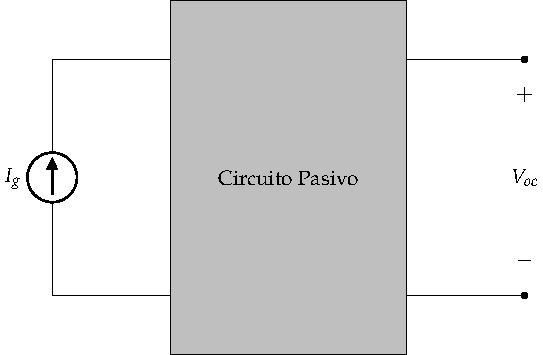
\includegraphics[height=4cm]{../figs/TeoremaReciprocidadCorriente1.pdf}\label{fig:teorema-reciprocidad-corriente1}}\hspace{2cm}
  \subfloat[Fuente de corriente en la salida]{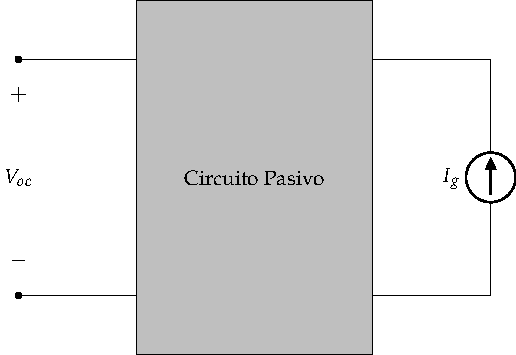
\includegraphics[height=4cm]{../figs/TeoremaReciprocidadCorriente2.pdf}\label{fig:teorema-reciprocidad-corriente2}}
  \caption{Teorema de reciprocidad aplicado a un circuito alimentado por una fuente de corriente.}
  \label{fig:teorema-reciprocidad-corriente}
\end{figure}

\subsection{Teorema de sustitución}
\label{sec:teorema-sustitucion}

Sea un circuito lineal (no necesariamente pasivo) en el que una rama cualquiera tiene una impedancia $Z$ (figura \ref{fig:teorema-sustitucion0}). Esta impedancia es recorrida por una corriente $I_Z$ y tiene una tensión $U_Z$, siendo $\overline{U}_Z = \overline{Z} \cdot \overline{I}_Z$. El teorema de sustitución indica que esta impedancia puede ser sustituida por una fuente de tensión cuya fuerza electromotriz sea $\overline{Z} \cdot \overline{I}_Z$ (figura \ref{fig:teorema-sustitucion-tension}), o por una fuente de corriente cuya corriente sea $\overline{U}_Z / \overline{Z}$ (figura figura \ref{fig:teorema-sustitucion-corriente}).


\begin{figure}[H]
  \centering
  \subfloat[Circuito original]{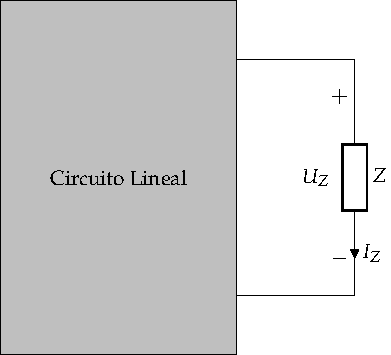
\includegraphics[height=4cm]{../figs/TeoremaSustitucion0.pdf}\label{fig:teorema-sustitucion0}}\\
  \subfloat[Sustitución con fuente de tensión]{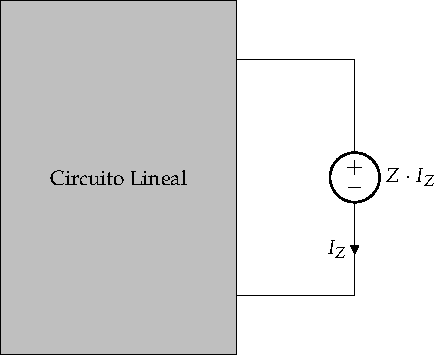
\includegraphics[height=4cm]{../figs/TeoremaSustitucionTension.pdf}\label{fig:teorema-sustitucion-tension}}\hspace{2cm}
  \subfloat[Sustitución con fuente de corriente]{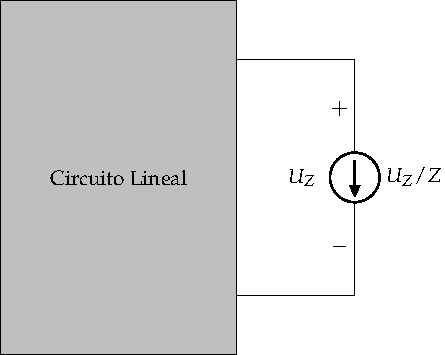
\includegraphics[height=4cm]{../figs/TeoremaSustitucionCorriente.pdf}\label{fig:teorema-sustitucion-corriente}}
  \caption{Teorema de sustitución.}
  \label{fig:teorema-sustitucion}
\end{figure}



\section{\textsuperscript{TC2} Teorema de compensación}
\label{sec:orgea27890}

El teorema de compensación permite calcular la variación que se produce en la respuesta de un circuito lineal cuando se modifica una de las impedancias que lo componen. Vamos a ilustrar este teorema mediante el circuito de la figura \ref{fig:teorema-compensacion0}, en el que se analizará la variación en la corriente $I_k$ (respuesta del circuito), $\Delta I_k$, ante la modificación de la impedancia $Z$, $\Delta Z$.


\begin{figure}[H]
  \centering
  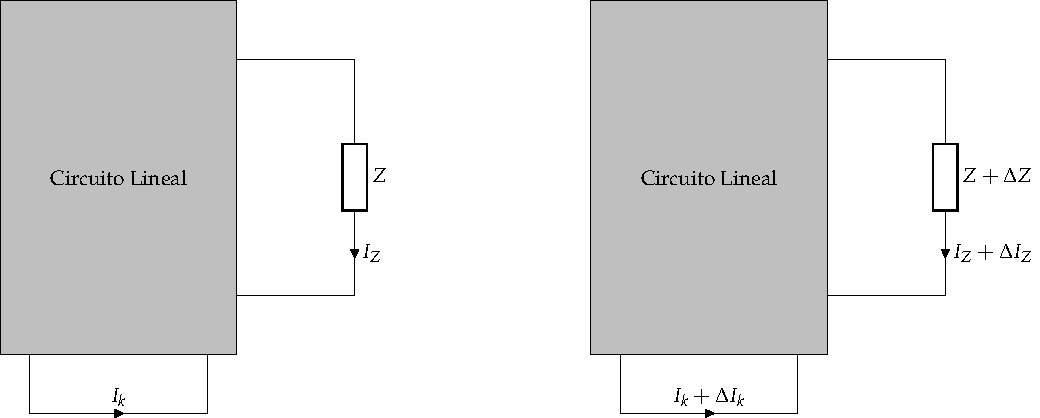
\includegraphics[height=4cm]{../figs/TeoremaCompensacion0.pdf}
  \caption{Teorema de la compensación: ¿cómo varía $I_k$ ante cambios en $Z$?}
  \label{fig:teorema-compensacion0}
\end{figure}


En primer lugar, separamos la impedancia modificada en dos impedancias en serie, la original, $Z$, y la modificación, $\Delta Z$. A esta última impedancia le aplicamos el teorema de sustitución, sustituyéndola por una fuente de tensión (figura \ref{fig:teorema-compensacion1}).

\begin{figure}[H]
  \centering
  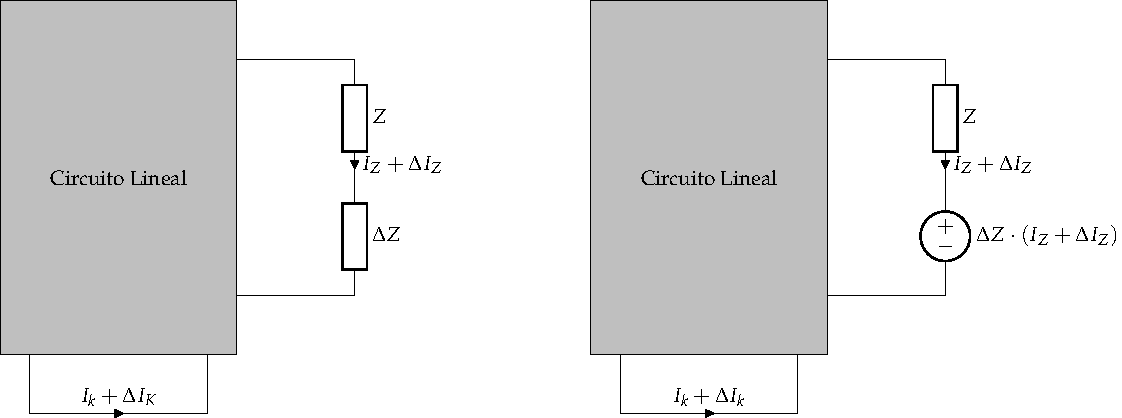
\includegraphics[height=4cm]{../figs/TeoremaCompensacion1.pdf}
  \caption{Teorema de compensación: aplicación del teorema de sustitución.}
  \label{fig:teorema-compensacion1}
\end{figure}

A continuación, podemos aplicar el teorema de superposición separando por una parte las fuentes presentes en el circuito y, por otra parte, la fuente resultante del teorema de sustitución, que estará conectada a un circuito pasivo (figura \ref{fig:teorema-compensacion2}). 

\begin{figure}[H]
  \centering
  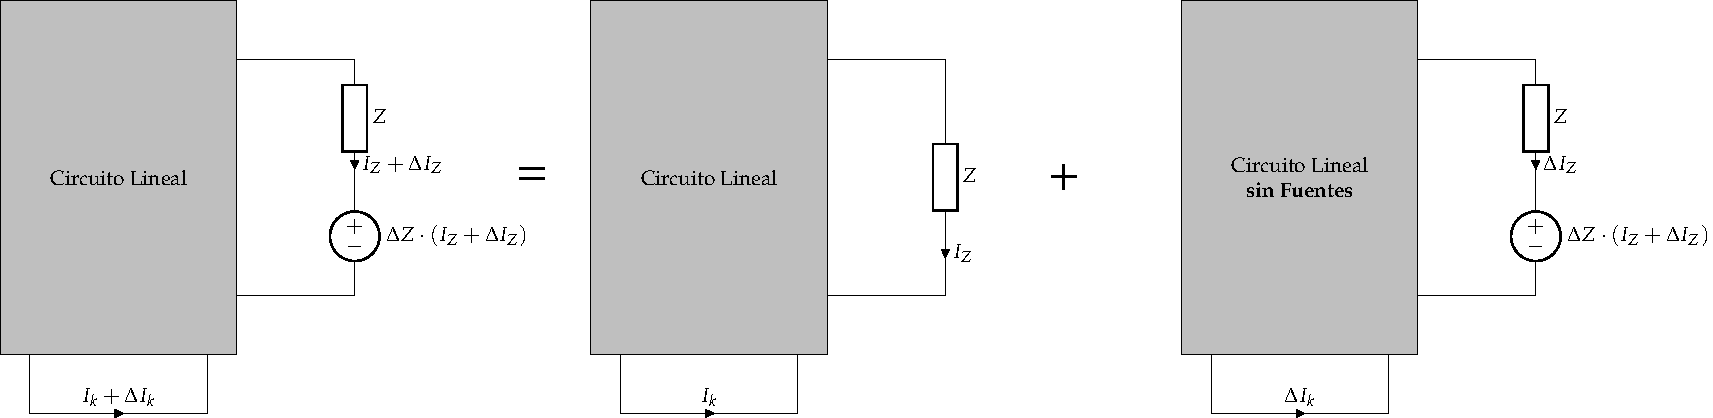
\includegraphics[height=4cm]{../figs/TeoremaCompensacion2.pdf}
  \caption{Teorema de compensación: aplicación del teorema de superposición.}
  \label{fig:teorema-compensacion2}
\end{figure}

En el último circuito, se puede expresar la fuente como:

\begin{equation}
  \Delta Z \cdot (I_Z + \Delta I_Z) = \Delta Z \cdot I_Z + \Delta Z \cdot \Delta I_Z
\end{equation}

El último sumando representa la tensión en la impedancia $\Delta Z$  recorrida por la corriente de la rama, $\Delta I_z$. Esta observación nos permite volver a utilizar el teorema de sustitución (figura \ref{fig:teorema-compensacion3}).

\begin{figure}[H]
  \centering
  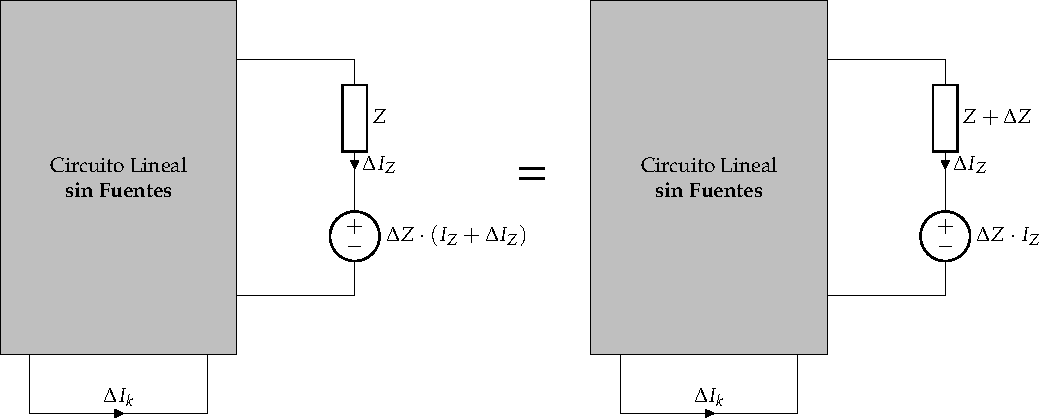
\includegraphics[height=4cm]{../figs/TeoremaCompensacion3.pdf}
  \caption{Teorema de compensación: nuevamente aplicación del teorema de sustitución.}
  \label{fig:teorema-compensacion3}
\end{figure}


Este resultado nos permite establecer el siguiente procedimiento de cálculo:

\begin{enumerate}
\item Se calcula la corriente $I_z$ en el circuito original (figura \ref{fig:teorema-compensacion-paso1}).
\item Se apagan las fuentes independientes y se sustituye la impedancia $Z$ por una impedancia de valor $Z + \Delta Z$ en serie con una fuente de tensión de valor $\Delta Z \cdot I_z$ (figura \ref{fig:teorema-compensacion-paso2}).
\item En el circuito resultante se calcula la respuesta, $\Delta I_k$. Esta corriente es la variación de la respuesta del circuito a la modificación de la impedancia (figura \ref{fig:teorema-compensacion-paso3}).
\end{enumerate}


\begin{figure}[H]
  \centering
  \subfloat[Circuito original]{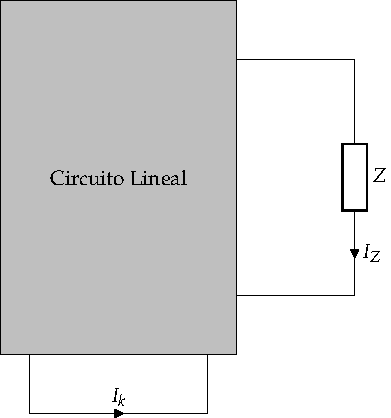
\includegraphics[height=4cm]{../figs/TeoremaCompensacion_Paso1.pdf}\label{fig:teorema-compensacion-paso1}}\hspace{1cm}
  \subfloat[Circuito de cálculo]{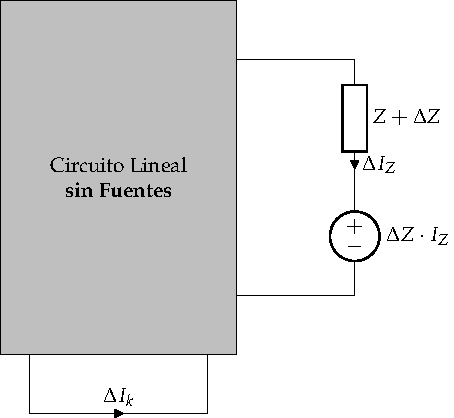
\includegraphics[height=4cm]{../figs/TeoremaCompensacion_Paso2.pdf}\label{fig:teorema-compensacion-paso2}}\hspace{1cm}
  \subfloat[Circuito modificado]{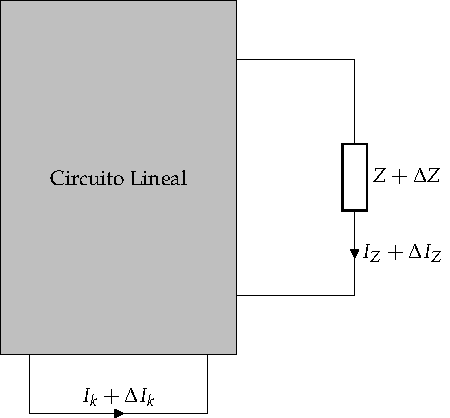
\includegraphics[height=4cm]{../figs/TeoremaCompensacion_Paso3.pdf}\label{fig:teorema-compensacion-paso3}}
  \caption{Procedimiento de cálculo del teorema de compensación.}
  \label{fig:teorema-compensacion-procedimiento}
\end{figure}



\section{\textsuperscript{TC2} Teorema de Millman}
\label{sec:teorema-millman}


El Teorema de Millman permite resolver la tensión entre dos puntos A y O de una red, siendo O un punto común de un conjunto de impedancias, y siendo conocidas las tensiones entre el punto A y las impedancias (figura \ref{fig:teorema-millman})

\begin{figure}[H]
  \centering
  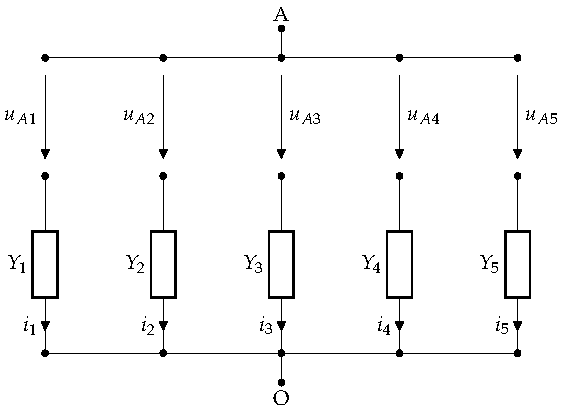
\includegraphics[height=5cm]{../figs/Millman.pdf}
  \caption{Teorema de Millman.}
  \label{fig:teorema-millman}
\end{figure}

En este circuito, la tensión $u_{AO}$ es:
\begin{equation}
  u_{AO} = u_{Aj} + i_j/Y_j
\end{equation}

Despejando $i_j$:

\begin{equation}
  i_j = Y_j \cdot (u_{AO} - u_{Aj})
\end{equation}

En el nudo O se puede plantear la LKC:

\begin{equation}
  \sum_{j = 1}^n i_j = 0
\end{equation}

Por tanto:
\begin{equation}
  \sum_{j = 1}^n Y_j \cdot (u_{AO} - u_{Aj}) = 0 \rightarrow \boxed{u_{AO} = \frac{\sum_{j = 1}^n Y_j u_{Aj}}{\sum_{i = 1}^n Y_j}}
\end{equation}

Este teorema permite resolver rápidamente circuitos como el de la figura \ref{fig:teorema-millman-aplicacion}, en el que una de las impedancias no tiene un generador asociado, actuando como carga del resto del circuito:

\begin{figure}[H]
  \centering
  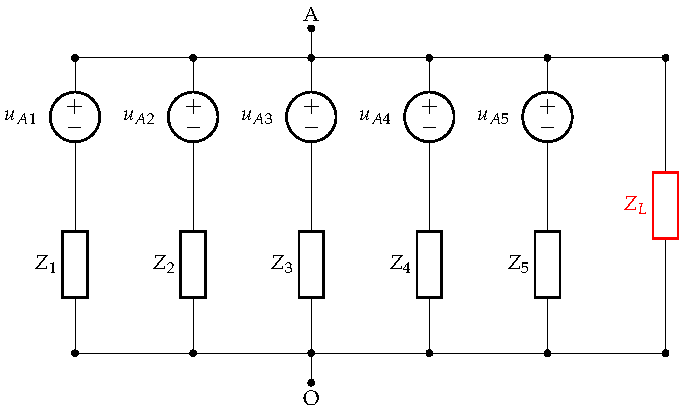
\includegraphics[height=5cm]{../figs/Millman_aplicacion.pdf}
  \caption{Aplicación del teorema de Millman}
  \label{fig:teorema-millman-aplicacion}
\end{figure}

En este caso, la tensión $u_{AO}$ es:

\begin{equation}
  u_{AO} = \frac{\sum_{j = 1}^5 u_{Aj}/Z_j}{{\color{red} 1/Z_L} + \sum_{i = 1}^5 1/Z_j}
\end{equation}

\section{\textsuperscript{TC2}  Teorema de Rosen}
\label{sec:teorema-rosen}

El teorema de Rosen permite transformar circuitos conectados en estrella (figura \ref{fig:teorema-rosen-estrella}) en circuitos poligonales (figura \ref{fig:teorema-rosen-poligono}):
\begin{figure}[H]
  \centering
  \subfloat[Conexión en estrella]{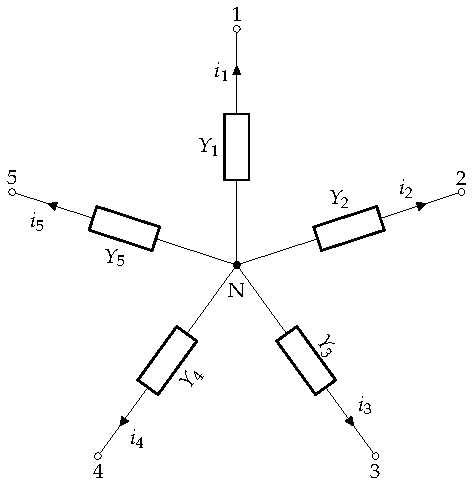
\includegraphics[height=5cm]{../figs/Rosen_Y.pdf}\label{fig:teorema-rosen-estrella}}\hspace{2cm}
  \subfloat[Conexión en polígono]{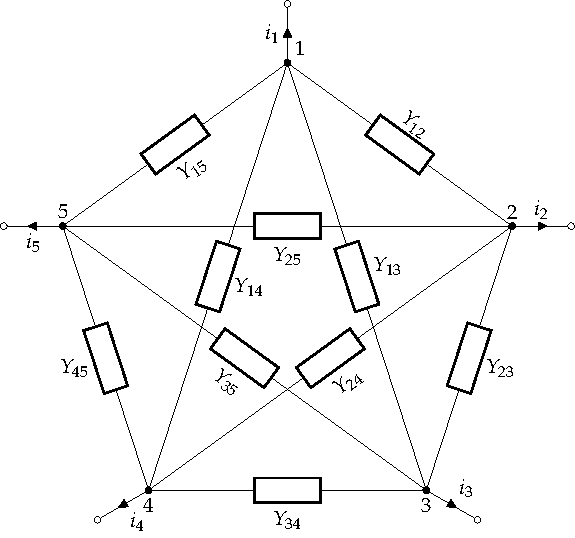
\includegraphics[height=5cm]{../figs/Rosen_D.pdf}\label{fig:teorema-rosen-poligono}}
  \caption{Teorema de Rosen}
  \label{fig:teorema-rosen}
\end{figure}

Para realizar la transformación debemos calcular las corrientes que salen por cada terminal en cada circuito. En el caso de la estrella, la corriente en cada rama es:
\begin{equation}
  i_j = Y_j \cdot u_{jN}
\end{equation}
Por su parte, la corriente de salida en conexión poligonal es:
\begin{equation}
  i_j = \sum_{\substack{k = 1\\k \neq j}}^n i_{kj} = \sum_{\substack{k = 1\\k \neq j}}^n u_{kj} \cdot Y_{kj} = \sum_{k = 1}^n u_{kj} \cdot Y_{kj}  
\end{equation}
teniendo en cuenta que $u_{kk} = 0$.

Para que los dos circuitos sean equivalentes, las ecuaciones de las corrientes deben dar el mismo resultado:

\begin{equation}
  Y_j \cdot u_{jN} = \sum_{k = 1}^n u_{kj} \cdot Y_{kj}  
\end{equation}

La tensión $u_{jN}$ de la estrella se puede relacionar con las tensiones entre terminales $u_{kj}$ a través del Teorema de Millman:

\begin{equation}
  u_{jN} = \frac{\sum_{k = 1}^n u_{kj} Y_k}{\sum_{k  = 1}^n Y_k}
\end{equation}

De esta forma, la relación entre estrella y polígono queda:
\begin{equation}
  \frac{\sum_{k = 1}^n u_{kj} Y_k Y_j}{\sum_{k  = 1}^n Y_k} = \sum_{k = 1}^n u_{kj} \cdot Y_{kj}  
\end{equation}

Podemos simplificar esta expresión denominando $Y_Y = \sum_{k  = 1}^n Y_k$ y agrupando dentro del sumatorio:
\begin{equation}
  \sum_{k = 1}^n u_{kj} \frac{Y_k Y_j}{Y_Y} = \sum_{k = 1}^n u_{kj} \cdot Y_{kj}  
\end{equation}

Por tanto, las admitancias de la conexión poligonal se pueden calcular a partir de las admitancias de la estrella con la ecuación \ref{eq:teorema-rosen}:

\begin{equation}
  Y_{kj} = \frac{Y_k Y_j}{Y_Y}
  \label{eq:teorema-rosen}
\end{equation}

Apliquemos este resultado a un ejemplo conocido, la transformación de una estrella ($n = 3$, figura \ref{fig:teorema-rosen-estrella3}) a un triángulo (figura \ref{fig:teorema-rosen-triangulo}). Sustituyendo en la ecuación anterior con las impedancias de la figura \ref{fig:teorema-rosen-aplicacion} obtenemos:

\begin{align*}
  Y_{ab} &= \frac{Y_a Y_b}{Y_a + Y_b + Y_c}\\
  \\
  Y_{bc} &= \frac{Y_b Y_c}{Y_a + Y_b + Y_c}\\
  \\
  Y_{ca} &= \frac{Y_c Y_a}{Y_a + Y_b + Y_c}\\
\end{align*}

\begin{figure}[H]
  \centering
  \subfloat[Conexión en estrella ($n = 3$)]{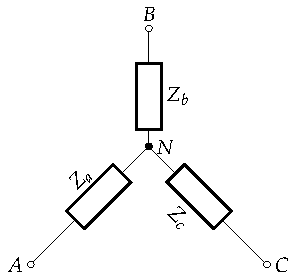
\includegraphics[height=4cm]{../figs/Impedancia_Estrella.pdf}\label{fig:teorema-rosen-estrella3}}\hspace{2cm}
  \subfloat[Conexión en triángulo]{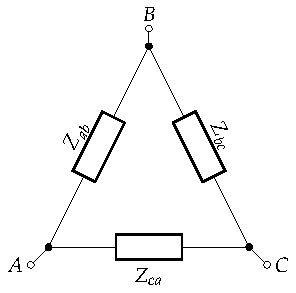
\includegraphics[height=4cm]{../figs/Impedancia_Triangulo.pdf}\label{fig:teorema-rosen-triangulo}}
  \caption{Aplicación del teorema de Rosen a una transformación estrella-triángulo.}
  \label{fig:teorema-rosen-aplicacion}
\end{figure}

\section{\textsuperscript{TC2} Teorema de Everitt}
\label{sec:org68c10d8}

El teorema de Everitt indica que si a la entrada de un circuito no disipativo (LC) existe adaptación de impedancias (la impedancia de entrada del circuito es $\overline{Z}_g^*$), a la salida de este circuito también se produce adaptación (la impedancia de salida es $\overline{Z}_L^*$) (figura \ref{fig:teorema-everitt}). Dado que, en general, el generador y la carga no están adaptados, $\overline{Z}_L \neq \overline{Z}^*_g$, el circuito no disipativo es una red adaptadora.

\begin{figure}[H]
  \centering
  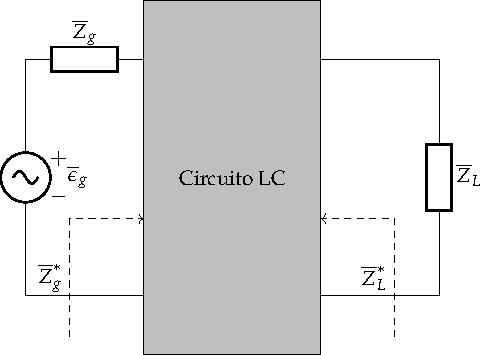
\includegraphics[height=5cm]{../figs/Everitt.pdf}
  \caption{Teorema de Everitt}
  \label{fig:teorema-everitt}
\end{figure}


Dado que un circuito LC no consume potencia activa, la potencia a la entrada es la potencia consumida por la carga $Z_L$ (figura \ref{fig:teorema-everitt-potencia}). Por tanto, si la potencia a la entrada es máxima (adaptación en la entrada), también lo será a la salida (adaptación a la salida).

\begin{figure}[H]
  \centering
  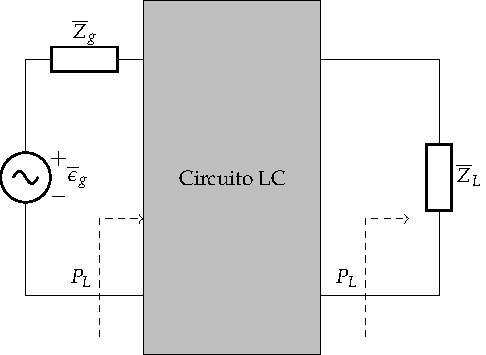
\includegraphics[height=5cm]{../figs/Everitt_potencia.pdf}
  \caption{Teorema de Everitt: potencia a la entrada y salida.}
  \label{fig:teorema-everitt-potencia}
\end{figure}

Este teorema también puede aplicarse a un conjunto de circuitos conectados en cascada (figura \ref{fig:teorema-everitt-cascada}). Si en una cascada de circuitos LC existe adaptación de impedancias en un punto de la cadena, existirá adaptación en cualquier punto de la misma.

\begin{figure}[H]
  \centering
  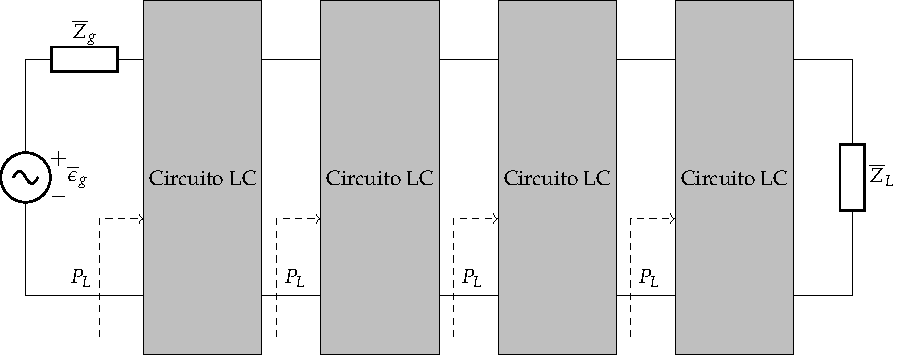
\includegraphics[height=5cm]{../figs/Everitt_cascada.pdf}
  \caption{Teorema de Everitt aplicado a una conexión en cascada.}
  \label{fig:teorema-everitt-cascada}
\end{figure}


\subsection{Diseño de redes adaptadoras}
\label{sec:everitt-diseño}

Una aplicación de este teorema es el diseño de redes adaptadoras
pasivas, para lo que emplearemos configuraciones en $\Gamma$ o
\reflectbox{$\Gamma$} compuestas por dos elementos reactivos (figura
\ref{fig:teorema-everitt-redes}):

\begin{figure}[H]
  \centering 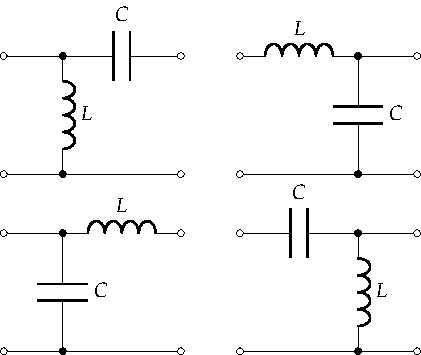
\includegraphics[height=5cm]{../figs/Everitt_LC.pdf}
  \caption{Redes adaptadoras pasivas en $\Gamma$ o
    \reflectbox{$\Gamma$}.}
  \label{fig:teorema-everitt-redes}
\end{figure}

El diseño de estas redes consiste en determinar los valores adecuados
de la inductancia y la capacidad para conseguir la adaptación de
impedancias. Es posible demostrar que, para obtener soluciones, la red
debe diseñarse con el elemento paralelo en el extremo de la impedancia
que tenga la parte real mayor. Cuando $R_g > R_L$, se optará por el
circuito de la figura \ref{fig:teorema-everitt-RG}, mientras que el
circuito de la figura \ref{fig:teorema-everitt-RL} será el adecuado
cuando $R_L > Rg$.

\begin{figure}[H]
  \centering \subfloat[Circuito adecuado para
  $R_g >
  R_L$]{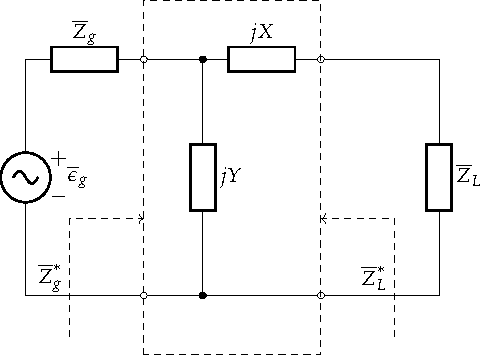
\includegraphics[height=4cm]{../figs/Everitt_XY2.pdf}\label{fig:teorema-everitt-RG}}\hspace{2cm}
  \subfloat[Circuito adecuado para
  $R_L >
  R_g$]{\includegraphics[height=4cm]{../figs/Everitt_XY1.pdf}\label{fig:teorema-everitt-RL}}
  \caption{Elección de la red adaptadora en función de la relación
    entre $R_L$ y $R_g$.}
  \label{fig:teorema-everitt-RLRG}
\end{figure}


Cuando $R_g > R_L$ la condición de adaptación se establece en la
salida de la red:
\begin{equation}
  \overline{Z}^*_L = jX + (jY || \overline{Z}_g) 
\end{equation}
Esta ecuación puede desdoblarse en otras dos:
\begin{align}
  R_L &= \Re\left(\frac{jY \cdot \overline{Z}_g}{jY + \overline{Z}_g}\right)\\
  X_L &= -X - \Im\left(\frac{jY \cdot \overline{Z}_g}{jY + \overline{Z}_g}\right)
\end{align}

Cuando $R_L > R_g$ la condición de adaptación se establece en la
entrada de la red:

\begin{equation}
  \overline{Z}^*_g = jX + (jY || \overline{Z}_L) 
\end{equation}
ecuación que, nuevamente, se desdobla en otras dos:
\begin{align}
  R_g &= \Re\left(\frac{jY \cdot \overline{Z}_L}{jY + \overline{Z}_L}\right)\\
  X_g &= -X - \Im\left(\frac{jY \cdot \overline{Z}_L}{jY + \overline{Z}_L}\right)
\end{align}

La resolución del sistema de ecuaciones en un caso o en otro
proporcionará los valores de $X$ e $Y$, que corresponden a las
reactancias de los elementos circuitales que componen la red
adaptadora (figura \ref{fig:teorema-everitt-redes}). Para obtener los
valores de inductancia y capacidad de los elementos a partir de estas
reactancias, será necesario recurrir a un valor de pulsación o
frecuencia. Por tanto, la adaptación conseguida con la bobina y el
condensador resultantes es selectiva, es decir, se produce para la
pulsación o frecuencia que se ha tenido en cuenta en el
cálculo. Cuando varíe la frecuencia del circuito dejará de haber
adaptación.

\subsection{Pérdidas de transmisión e inserción}
\label{sec:everitt-perdidas}

La inserción de una red dentro de un circuito existente modifica el
funcionamiento de este circuito y puede ocasionar pérdida o ganancia
en las señales de tensión, corriente y potencia en la inserción. Para
cuantificar estas variaciones se calcula la ratio entre los dos
niveles de la magnitud en estudio.

Frecuentemente el cálculo se efectúa en unidades logarítmicas. Sean
$x_1$ y $x_2$ los dos niveles de la magnitud $x$ de interés. La
expresión \ref{eq:decibelio} cuantifica la ganancia de $x$ (ratio de
$x_2$ frente a $x_1$) en decibelios:

\begin{equation}
  \label{eq:decibelio}
  G_X = 10 \log \frac{x_2}{x_1}
\end{equation}

Cuando se trata de una ganancia, $x_2 > x_1$, será
$G_X > \qty{0}{\decibel}$. Por el contrario, cuando se trate de una
pérdida, $x_2 < x_1$, obtendremos $G_X < \qty{0}{\decibel}$. Por
ejemplo, el valor $G_X = \qty{3}{\decibel}$ implica que
$x_2 = 2 \cdot x_1$, mientras que si $G_X = - \qty{3}{\decibel}$, será
$x_2 = 1/2 \cdot x_1$, y cuando $x_2 = x_1$, la ganancia es nula,
$G_X = \qty{0}{\decibel}$,

En circuitos eléctricos se emplea esta unidad para la ganancia de
potencia (ecuación \ref{eq:ganancia-potencia}). También puede
emplearse para la ganancia de tensión o de corriente, aunque en este
caso la ecuación debe modificarse para tener en cuenta la relación
cuadrática entre estas magnitudes y la potencia (ecuación
\ref{eq:ganancia-tension}).

\begin{align}
  G_{dB} = 10 \log G &= 10 \log \frac{P_2}{P_1} \label{eq:ganancia-potencia}\\
  G_{dB} = 10 \log \frac{U_2^2}{U_1^2} &= 20 \log \frac{U_2}{U_1}   \label{eq:ganancia-tension}
\end{align}

Por tanto, una ganancia de $\qty{3}{\decibel}$ en potencia significa
que $P_2 = 2 \cdot P_1$, mientras que $U_2 = 2 \cdot U_1$ es una
ganancia de $\qty{6}{\decibel}$ en tensión.

Aplicaremos estos conceptos al cálculo de las pérdidas de transmisión y las pérdidas de inserción que se producen al introducir redes en un circuito.

\subsubsection{Pérdidas de Transmisión}
\label{sec:perdidas-transmision}

Las pérdidas de transmisión, $\alpha_T$, asociadas a una red miden la
relación entre la potencia de entrada, $P_{in}$, y la potencia de
salida, $P_{out}$ (figura \ref{fig:perdidas-transmision}).

\begin{figure}[H]
  \centering
  \includegraphics[height=4cm]{../figs/PerdidasTransmision.pdf}
  \caption{Pérdidas de transmisión.}
  \label{fig:perdidas-transmision}
\end{figure}

\begin{equation}
  \alpha_T = 10 \log \frac{P_{in}}{P_{out}} \unit{\decibel}
\end{equation}

Si la red es no disipativa, $P_{in} = P_{out}$ y, por tanto, las
pérdidas de transmisión son nulas, $\alpha_T = \qty{0}{\decibel}$. Si la red es disipativa, $P_{out} < P_{in}$ y, por tanto, $\alpha_T > \qty{0}{\decibel}$. Finalmente, si la red es activa puede ser que $P_{out} > P_{in}$ y, por tanto, $\alpha_T < \qty{0}{\decibel}$, lo que implica una \emph{ganancia} de transmisión.

\subsubsection{Pérdidas de inserción}
\label{sec:perdidas-insercion}

Las pérdidas de inserción asociadas a una red, $\alpha_I$, miden la
relación entre la potencia entregada a la carga sin la red, $P_L$, y
la potencia entregada a la carga con la red insertada (figura
\ref{fig:perdidas-insercion}).

\begin{figure}[H]
  \centering
  \includegraphics[height=4cm]{../figs/PerdidasInsercion.pdf}
  \caption{Pérdidas de inserción.}
  \label{fig:perdidas-insercion}
\end{figure}

\begin{equation}
  \alpha_I = 10 \log \frac{P_L}{P_{out}} \unit{\decibel}
\end{equation}

Al estar definida como pérdida, se está asumiendo que la inserción de
la red disminuye la potencia entregada a la carga. Ahora bien, en el
caso de una red adaptadora el efecto es el contrario, $P_{out} > P_L$,
por lo que $\alpha_I < 0$, siendo, por tanto, una \emph{ganancia} de
inserción.

%%% Local Variables:
%%% mode: latex
%%% TeX-master: "TC"
%%% ispell-local-dictionary: "castellano"
%%% End:
